\begin{pa} \label{PA:12.1}
It's common for weather forecasters to discuss the wind \emph{speed}, but as any student who has gotten this far in the text will know, this nomenclature is imprecise. It's not terribly helpful to tell someone the wind is blowing at $10$ km/h without telling them the direction in which the wind is blowing. If you're trying to make a decision based on what the wind is doing, you need to know about the direction as well. (Perhaps you are taking off in a hot air balloon and need to know which direction the chase team should head to keep track of you.) Because of the swirling nature of wind, it makes sense to give the wind \emph{velocity} at every point in a region (two-dimensional or three-dimensional). 

\ba
\item \label{enum:PA12.1F} Suppose that given a point $(x,y)$ in the plane, you know that the wind velocity at that point is given by the vector $\vF(x,y) = \langle y,x\rangle$. For example, we'd then know that at the point $(1,-1)$, the wind velocity is $\vF(1,-1) = \langle -1,1\rangle$. In the table below, fill in the wind velocity vectors for the given points.
  \begin{center}
    \begin{tabular}{c|c|c|c|c|c}
      $(x,y)$ & $(2,1)$ & $(0,0)$ & $(-1,2)$ & $(3,-1)$ & $(-2,-1)$\\\hline
$\vF(x,y)$ & & & & &
    \end{tabular}
  \end{center}
\item \label{enum:PA12.1G} Suppose that we associate the vector $\vG(x,y) = -x\vj$ to a point $(x,y)$ in the plane. Complete the table below by giving the vector associated to each of the given points.
  \begin{center}
    \begin{tabular}{c|c|c|c|c|c|c|c|c}
      $(x,y)$ & $(-2,0)$ & $(-1,2)$ & $(0,-2)$ & $(1,1)$ & $(2,3)$ & $(3,2)$ & $(-1,0)$ & $(1,3)$\\\hline
$\vG(x,y)$ & & & & & & &
    \end{tabular}
  \end{center}

\saveCount
\ea

A table of values of these vector-valued functions is useful, but perhaps even better is a method of visualizing the vectors. In keeping with our wind velocity analogy, if $\vF(2,1) = \langle 1,2\rangle$, we draw the vector $\langle 1,2\rangle$ with its tail at the point $(2,1)$. 

\ba
\restoreCount
\item Using the first set of axes in Figure~\ref{fig:PA12.1a}, plot the vectors $\vF(x,y)$ for the five points in the table in part \ref{enum:PA12.1F}. The example $\vF(1,-1) = \langle -1,1\rangle$ is drawn for you.
\item Using the second set of axes in Figure~\ref{fig:PA12.1a}, plot the vectors $\vG(x,y)$ for the eight points in the table in part \ref{enum:PA12.1G}. 
% TODO: Actually include the promised vector on the left grid.
  \begin{figure}[h]
    \centering
    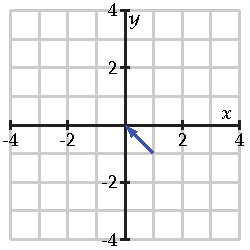
\includegraphics{figures/PA12-1F-axes.pdf}\hspace{0.5in}    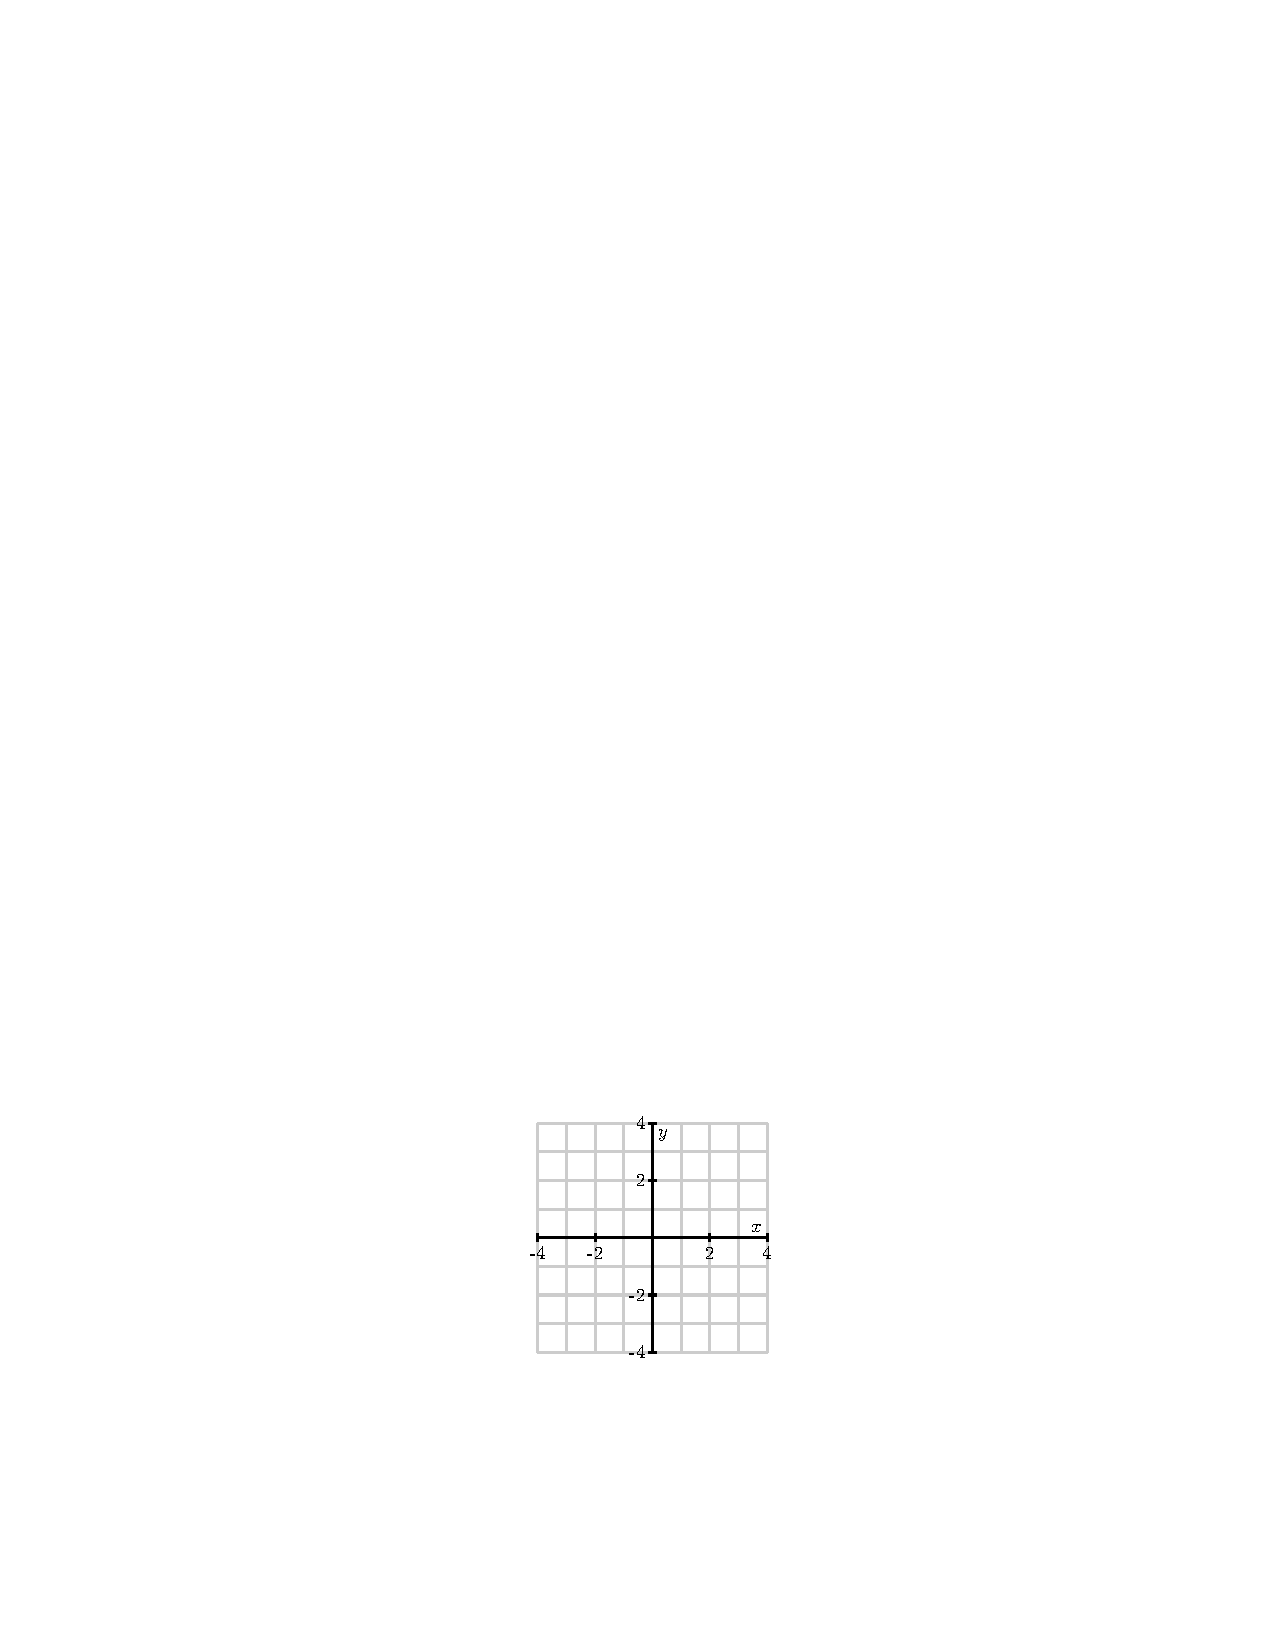
\includegraphics{figures/PA12-1G-axes.pdf}
    \caption{Axes for plotting some vectors from $\vF(x,y)$ and $\vG(x,y)$.}
    \label{fig:PA12.1a}
  \end{figure}
\ea
\end{pa} 
\afterpa 
%%% Local Variables:
%%% mode: latex
%%% TeX-master: "../0_AC_MV"
%%% End:
